We executed our experiments on PyCharm, an integrated development environment (IDE) dedicated primarily to the Python language, developed by JetBrains. We chose PyCharm because it has researcher-friendly functions such as version control for Python, debugging mode, and code self-completion~\citep{JetBrains2022}.


\subsection{Experiment A——Morphology and HSV based Algorithm}

\subsubsection{Determination of HSV Values}
By observing the dataset, we found that the colour of apples come not only in red, but also in orange and yellow, so we adjusted the H-values to ranges of red, orange and yellow, which are $[0, 34]$ and $[156, 180]$. As for green apples, we set it to $[78, 90]$ through several experiments when the best performance occurred. Except for the black, gray and white, S-values were fixed in the range of $[43, 255]$. Furthermore, Due to factors such as lighting and shading on the apples, we increased the range of V-value to $[15, 255]$. 

\subsubsection{Determination of the Size and Shape of the Mask Kernel}
Though the apples with various colours can be detected, we found that the apples on distant tree are difficult to identify due to their excessively small size (Fig.~\ref{fig:detected_before_after}(a)).

\begin{figure}[!htb]
    \centering
    \subfigure[Detected apples before the modification of the kernel size]{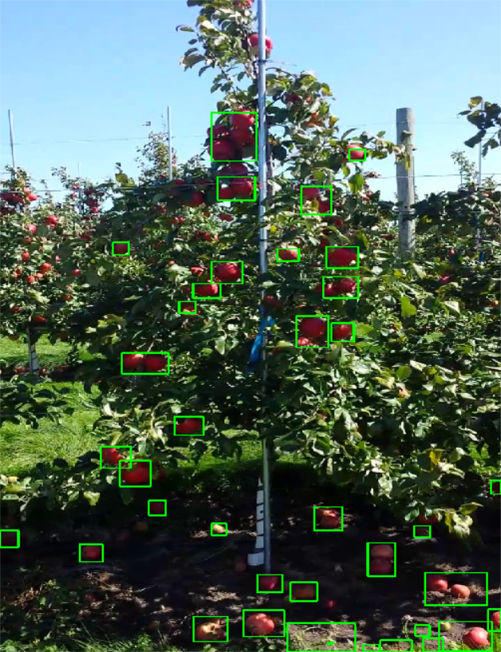
\includegraphics[width=0.35\textwidth]{images/detection_before.png}}
    \subfigure[Detected apples after the modification of the kernel size]{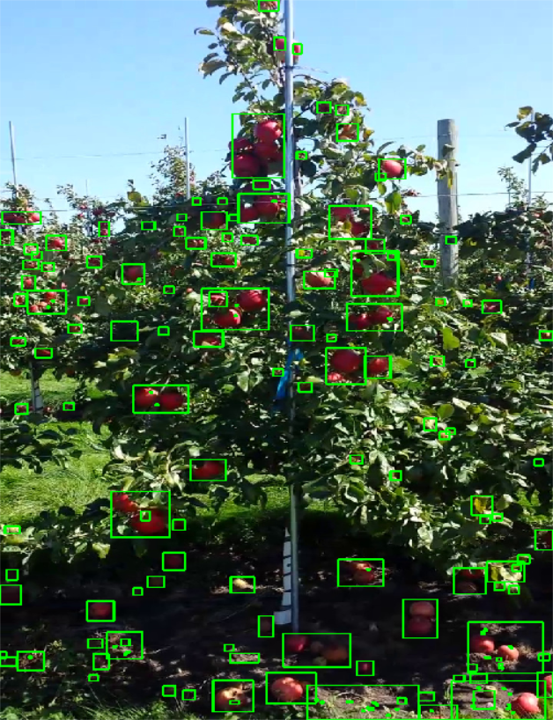
\includegraphics[width=0.35\textwidth]{images/detection_after.png}}
    \caption{Detected apples before and after the modification of the kernel size——(a) before the modification and (b) after the modification}
    \label{fig:detected_before_after}
\end{figure}

To capture the apples of small size, we adjusted the size of the mask for inRange thresholding, and we tried different sizes from $5\times 5$ to $1\times 1$, as shown in Fig.~\ref{fig:diff_mask_kernelsize}. When the kernel size is $3\times 3$, most of the apples can be counted and the noise can be effectively removed. Moreover, we chose ‘MORPH\_ELLIPSE’ as the shape of the kernel as most of the apples are oval in shape.

\begin{figure}[htb]
    \centering
    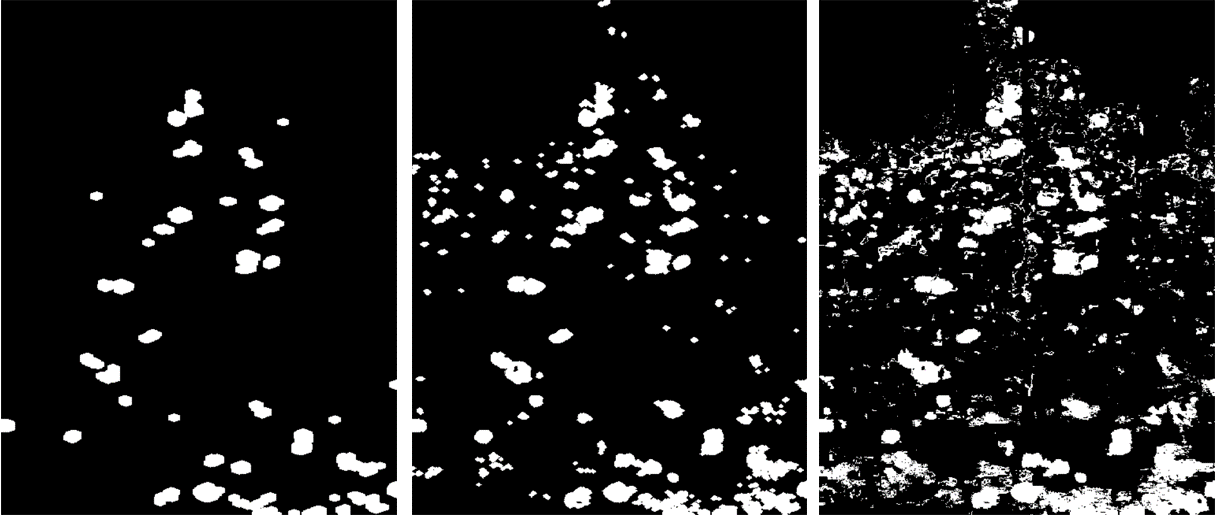
\includegraphics[width=0.65\textwidth]{images/diff_kernel_size.png}
    \caption{Processed images by masks with a kernel size of $5\times 5$ (left), $3\times 3$ (middle) and $1\times 1$ (right)}
    \label{fig:diff_mask_kernelsize}
\end{figure}

\subsubsection{Determination of the Values in Opening}
\begin{itemize}
    \item \textbf{Kernel size.} The opening operations smooth out noise and reduce the size of small objects in the image, while preserving larger features. The kernel is applied to the masked images using the 'morphologyEx()' function with the 'MORPH\_OPEN' flag. Since its computational principle is convolution, which is the same as that of inRange thresholding in the previous subsection, we set the size of the kernel for the opening to $3\times 3$.
    % The erosion operation shrinks the white regions of the image by applying a structuring element and setting a pixel to white only if all pixels under the structuring element are also white. This has the effect of eroding away small white features and leaving larger features intact. The dilation operation expands the white regions of the image by applying the structuring element and setting a pixel to white if any pixel under the structuring element is white. This has the effect of restoring larger white features that were eroded by the erosion operation and filling in gaps between white features. Together, 
    
    \item \textbf{Number of iterations.} A large number of iterations will result in aggressive smoothing and noise reduction, but may also result in the loss of small features in the image, while the opposite is true for a small number of iterations. We tried iteration times from 1 to 10, as shown in Fig.~\ref{fig:diff_iteration_times}. When the times of iterations is 5, the image has the optimal smoothing and noise reduction.
    
        \begin{figure}[htb]
                \centering
                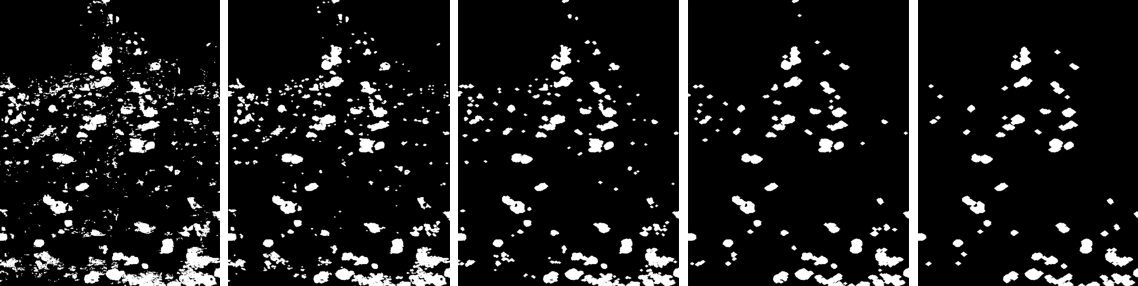
\includegraphics[width=0.95\textwidth]{images/iteration.png}
                \caption{Processed images with different numbers of iteration——1 (left), 3 (middle left), 5 (middle), 7 (middle right), 9 (right)}
                \label{fig:diff_iteration_times}
        \end{figure}
    
\end{itemize}



\subsubsection{Determination of the Threshold for Contours' Area}
As shown in Fig.~\ref{fig:contour_modified}, some of the contours with too small size did not contain apples. So, we used ‘contourArea’ to screen off the contours whose areas are smaller than 200. After the series of operations, most of the apples in the images can be captured.

\begin{figure}[!ht]
    \centering
    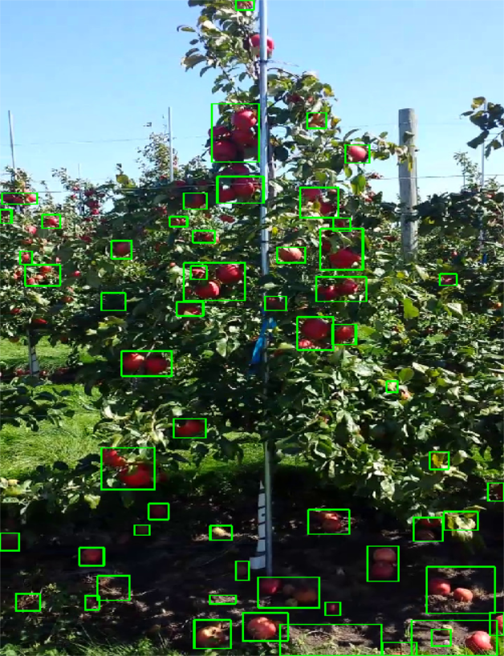
\includegraphics[width=0.4\textwidth]{images/detection_contours_outcome.png}
    \caption{Detected apples after the modification of the threshold for the contours' area}
    \label{fig:contour_modified}
\end{figure}

\subsection{Experiment B——Deep Learning}

\subsubsection{Dataset preparation}
Unlike the traditional approach of identifying apples, deep learning requires a training set, which we mentioned at Section~\ref{sec:Data}. The detection training dataset contains 670 images and the corresponding images in the form of Mask, as well as 331 test images (Fig.~\ref{fig:masked_detection_image}). 

\subsubsection{Pre-processing of the Dataset}
As the annotations in the detection training set are in masks, they need to be converted to the same type of XML tag data as the VOC2007 data tags to make them compatible with YOLO. For this purpose, we used OpenCV to convert the label of the dataset.

To facilitate the recognition process, we used python to uniformly process all training set images and annotated images to a size of $640\times 640$. OpenCV was then called to read the mask maps, taking the upper and left boundaries of each grey-scale value as the starting point of the labelled box, and the right and lower boundaries were calculated with the starting point to obtain the width and height of the box. The data from each mask image is then processed and written to XML to obtain a YOLO-compatible data label. 




\subsubsection{Training}
The hardware used to train YOLOX and the training hyperparameters are listed in Tab.~\ref{tab:Hyperparameters} and Tab.~\ref{tab:Hardwares} respectively. We completed the training with Python 3.8, corresponding to PyTorch and CUDA versions 1.9.0 and 11.1.

\begin{table}[htb]
\centering
\caption{Hardwares and their parameters}
\label{tab:Hardwares}
\resizebox{\textwidth}{!}{%
\begin{tabular}{@{}p{7cm}<{\centering} p{7cm}<{\centering}@{}}
\toprule
Hardware & Parameter                       \\ \midrule
GPU      & NVIDIA $A40 \times 1$           \\
VRAM     & $48\ GB$                        \\
CPU      & AMD EPYC 7543 32-Core Processor \\
RAM      & $80\ GB$                        \\ \bottomrule
\end{tabular}%
}
\end{table}

\begin{table}[htb]
\centering
\caption{Hyperparameters for training}
\label{tab:Hyperparameters}
\resizebox{\textwidth}{!}{%
\begin{tabular}{@{}p{7cm}<{\centering} p{7cm}<{\centering}@{}}
\toprule
Hyperparameter        & Value        \\ \midrule
Input shape           & $[640, 640]$ \\
Epoch                 & 300          \\
Freeze\_Epoch         & 50           \\
Batch size            & 16           \\
Freeze\_batch\_size   & 64           \\
Initial learning rate  & 0.01         \\
Minimum learning rate & 0.0001       \\
Optimizer             & SGD          \\
Activation function   & SiLU \\ \bottomrule
\end{tabular}%
}
\end{table}

In order to improve efficiency, we experimented with freeze training. Freeze training is an idea of migration learning, which is widely encountered in target detection tasks. Since the features extracted from the backbone of a target detection model are generic, freezing the backbone speeds up training and prevent the weights from being corrupted. In the freeze phase, the backbone of the model is frozen and the feature extraction network remains unchanged, taking up less memory, at which point we can fine-tune the network structure. In the unfreeze phase, the feature extraction network is adaptable, occupying more memory and all of the parameters are changed. Therefore, we set the batch size to be larger in the freezing phase and smaller in the thawing phase. We freeze the network in the first 50 epochs and thaw it in the last 250 epochs.

The curve of the loss and the mean Average Precision (mAP) along epochs is shown in Fig.~\ref{fig:Loss and mAP}. After 300 epochs, the loss in the validation dataset and the loss in the training dataset are both reduced to less than 3\%.

\begin{figure}[htb]
    \centering
    \subfigure[Loss over epochs]{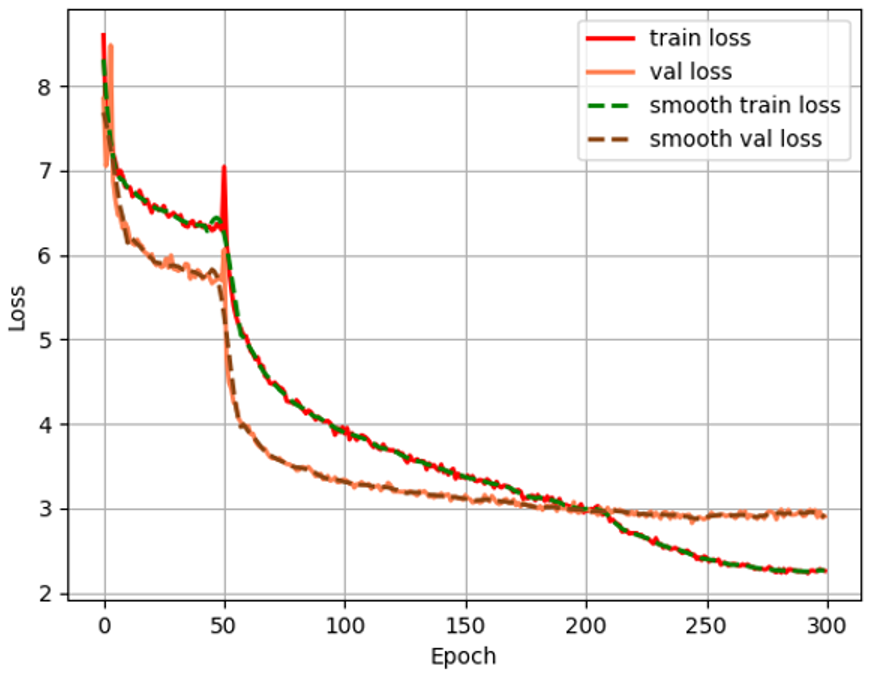
\includegraphics[width=0.49\textwidth]{images/Loss.png}}
    \subfigure[mAP over epochs]{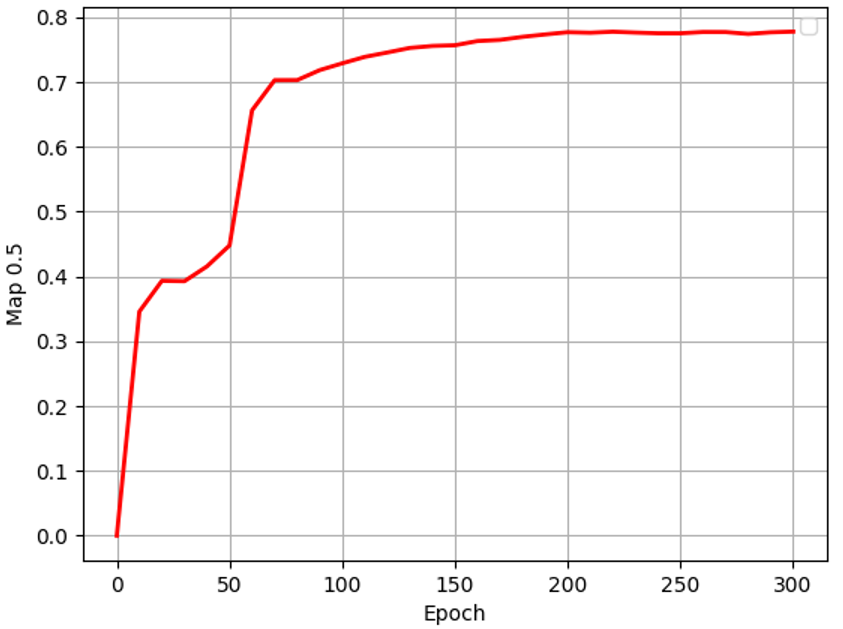
\includegraphics[width=0.5\textwidth]{images/MAP.png}}
    \caption{Loss and mAP over epochs}
    \label{fig:Loss and mAP}
\end{figure}
